\documentclass[final]{beamer}

\usepackage[scale=1.24]{beamerposter} % Use the beamerposter package for laying out the poster

\usetheme{confposter}

\setbeamercolor{block title}{fg=ngreen,bg=white} % Colors of the block titles
\setbeamercolor{block body}{fg=black,bg=white} % Colors of the body of blocks
\setbeamercolor{block alerted title}{fg=white,bg=dblue!70} % Colors of the highlighted block titles
\setbeamercolor{block alerted body}{fg=black,bg=dblue!10} % Colors of the body of highlighted blocks
\addtobeamertemplate{block begin}{\setlength\abovedisplayskip{0pt}}

%-----------------------------------------------------------
% Define the column widths and overall poster size
% To set effective sepwid, onecolwid and twocolwid values, first choose how many columns you want and how much separation you want between columns
% In this template, the separation width chosen is 0.024 of the paper width and a 4-column layout
% onecolwid should therefore be (1-(# of columns+1)*sepwid)/# of columns e.g. (1-(4+1)*0.024)/4 = 0.22
% Set twocolwid to be (2*onecolwid)+sepwid = 0.464
% Set threecolwid to be (3*onecolwid)+2*sepwid = 0.708

\newlength{\sepwid}
\newlength{\onecolwid}
\newlength{\twocolwid}
\newlength{\threecolwid}
\newlength{\figwid}
\setlength{\paperwidth}{48in} % A0 width: 46.8in
\setlength{\paperheight}{36in} % A0 height: 33.1in
% \setlength{\sepwid}{0.024\paperwidth} % Separation width (white space) between columns
\setlength{\sepwid}{1ex} % Separation width (white space) between columns
% \setlength{\onecolwid}{0.32\paperwidth} % Width of one column
\setlength{\onecolwid}{0.32\paperwidth} % Width of one column
\setlength{\twocolwid}{0.464\paperwidth} % Width of two columns
\setlength{\threecolwid}{0.708\paperwidth} % Width of three columns
\setlength{\topmargin}{-0.5in} % Reduce the top margin size
\setlength{\figwid}{.6\onecolwid}
%-----------------------------------------------------------

\usepackage{graphicx}  % Required for including images

\usepackage{booktabs} % Top and bottom rules for tables




%----------------------------------------------------------------------------------------
%	TITLE SECTION
%----------------------------------------------------------------------------------------

\title{Research Title} % Poster title

\author{J. Russo, JJ Dong} % Author(s)

\institute{Bucknell University, Department of Physics and Astronomy} % Institution(s)


\begin{document}

% \addtobeamertemplate{block end}{}{\vspace*{1ex}} % White space under blocks
% \addtobeamertemplate{block alerted end}{}{\vspace*{1ex}} % White space under highlighted (alert) blocks

\setlength{\belowcaptionskip}{2ex} % White space under figures
\setlength\belowdisplayshortskip{2ex} % White space under equations




\begin{frame}[t] % The whole poster is enclosed in one beamer frame

\begin{block}

\begin{columns}[t] % The whole poster consists of three major columns, the second of which is split into two columns twice - the [t] option aligns each column's content to the top
\begin{column}{4ex}\end{column} % Empty spacer column

% ------------------------- First column -------------------------
\begin{column}{\onecolwid}

  %-------------
  %	Motivation
  %-------------
  \begin{alertblock}{Introduction}
  \begin{itemize}
    \item Ubiquitous threat of antibiotic resistant bacteria
    \item Investigate effect of different cellular transformation rates on antibiotic
    resistant bacterial population growth
  \end{itemize}

  \begin{center}
    Diagram of cell with plasmids
  \end{center}
  \end{alertblock}
\end{column}

% ----------------------------------------------------------------
\begin{column}{\sepwid}\end{column} % Empty spacer column

% ------------------------- Second column -------------------------
\begin{column}{.8\onecolwid}
  %-------------
  %	INTRODUCTION
  %-------------
  \begin{alertblock}{Biological Background}
    \begin{itemize}
      \item Plasmids
      \item Fitness cost
      \item Transformation
    \end{itemize}
  \end{alertblock}
\end{column}

\begin{column}{\sepwid}\end{column} % Empty spacer column

% ------------------------- Third column -------------------------
\begin{column}{\onecolwid}
  %-------------
  %	Motivation
  %-------------
  \begin{alertblock}{Simulation Methods}
    \begin{itemize}
      \item Combined approach of Kinetic Monte Carlo simulation and numerical modeling
      \item Gillespie algorithm
      \item Well-mixed population
      \item Carrying capacity
      \item Constant, Linear, Recycled $\alpha$
      \item Symmetric division
    \end{itemize}
  \end{alertblock}
\end{column}
% ----------------------------------------------------------------
% \begin{column}{\sepwid}\end{column} % Empty spacer column
\end{columns} % End of all the columns in the poster
\end{block}


\begin{block}

\begin{columns}[t]
% \begin{column}{\sepwid}\end{column} % Empty spacer column

% ------------------------- First column -------------------------
\begin{column}{\onecolwid}

  \setbeamercolor{block title}{fg=black,bg=white} % Colors of the block titles
  \begin{block}{Constant $\alpha$}
  \setbeamercolor{block title}{fg=ngreen,bg=white} % Colors of the block titles
  \begin{center}
    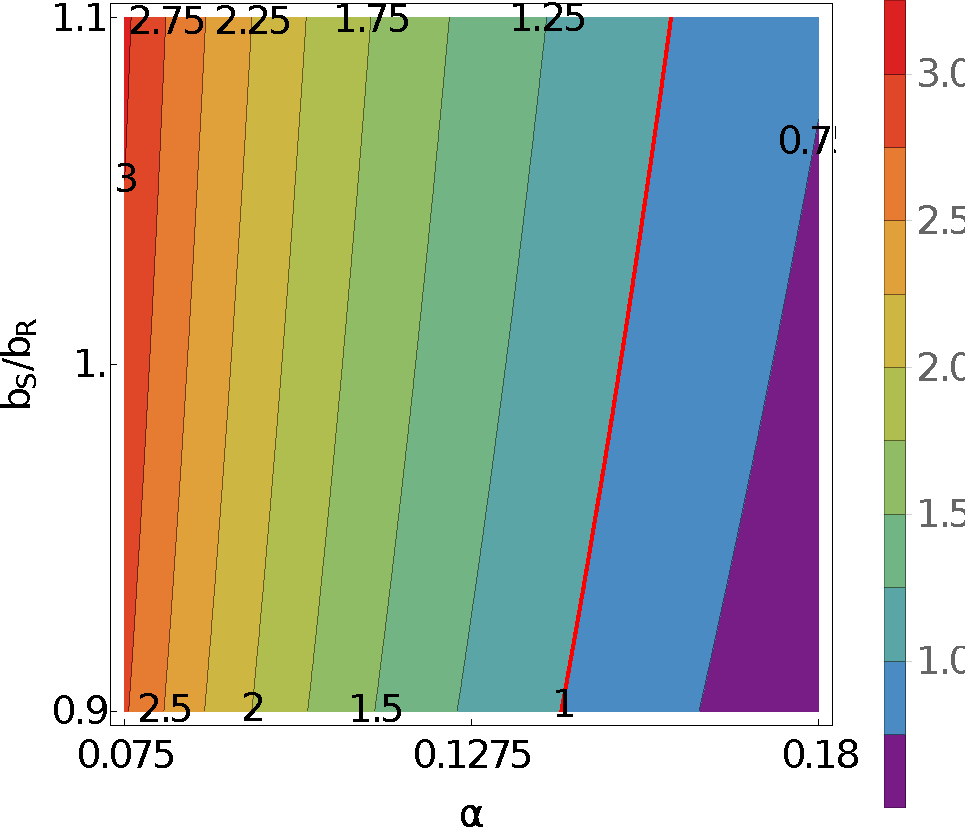
\includegraphics[width=\figwid]{../dev/graphics/poster/const_contour.pdf}

    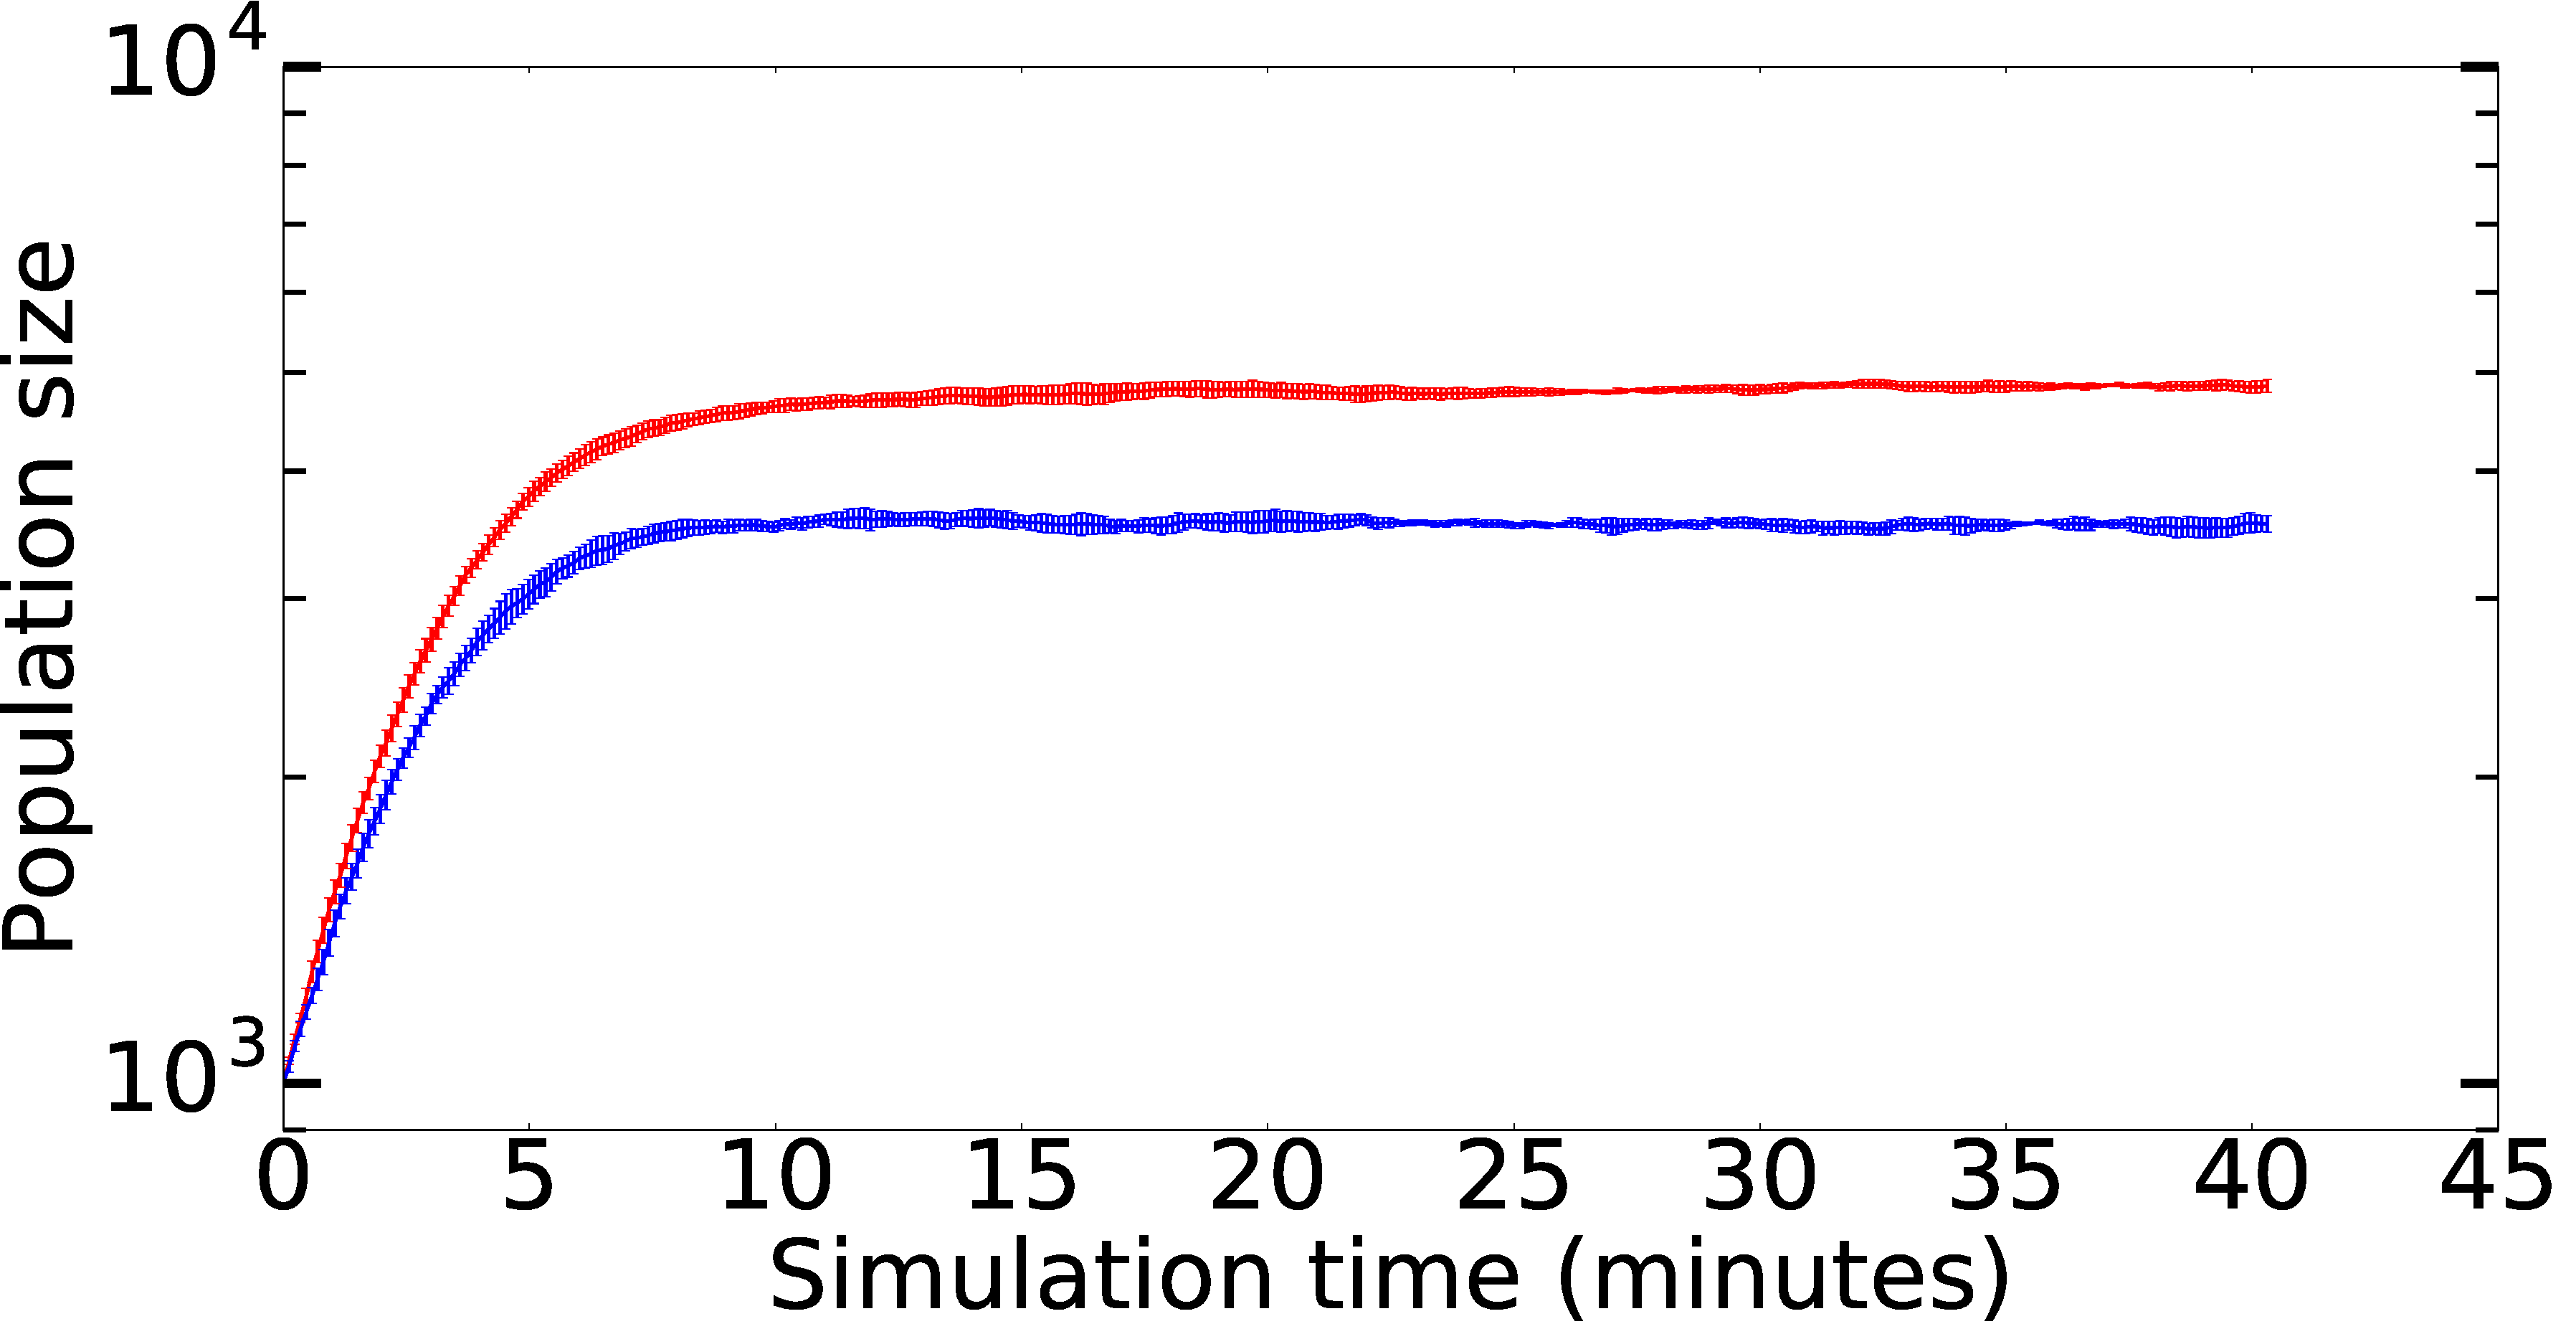
\includegraphics[width=\figwid]{../dev/graphics/poster/const_pop.pdf}
  \end{center}

  \begin{columns}[t]
    \begin{column}{.2\onecolwid}
      \begin{center}
        Reactions
      \end{center}
      \begin{align*}
        S & \stackrel{b_S}{\rightarrow} 2S \\
        S & \stackrel{\alpha}{\rightarrow}  R \\
        R & \stackrel{b_R}{\rightarrow} 2R \\
        R & \stackrel{\delta}{\rightarrow} \varnothing
      \end{align*}
    \end{column}
      \vrule
    \begin{column}{.5\onecolwid}
      \begin{center}
        Equations
      \end{center}

      \begin{align*}
        \frac{dS}{dt}& = \mu_1 \left(1 - \frac{S + R}{K}\right)S - \alpha S \\[0.5ex]
        \frac{dR}{dt}& = \mu_2 \left(1 - \frac{S + R}{K}\right)R + \alpha S - \delta R
      \end{align*}

      \vspace{.9\baselineskip}
      \vspace{.9\baselineskip}
    \end{column}
  \end{columns}

  \end{block}
\end{column}

% ----------------------------------------------------------------
\vrule width 5pt
\begin{column}{\sepwid}\end{column} % Empty spacer column

% ------------------------- Second column -------------------------
\begin{column}{\onecolwid}

  \setbeamercolor{block title}{fg=nred,bg=white} % Colors of the block titles
  \begin{block}{Linear $\alpha$}
  \setbeamercolor{block title}{fg=ngreen,bg=white} % Colors of the block titles
    \begin{center}
      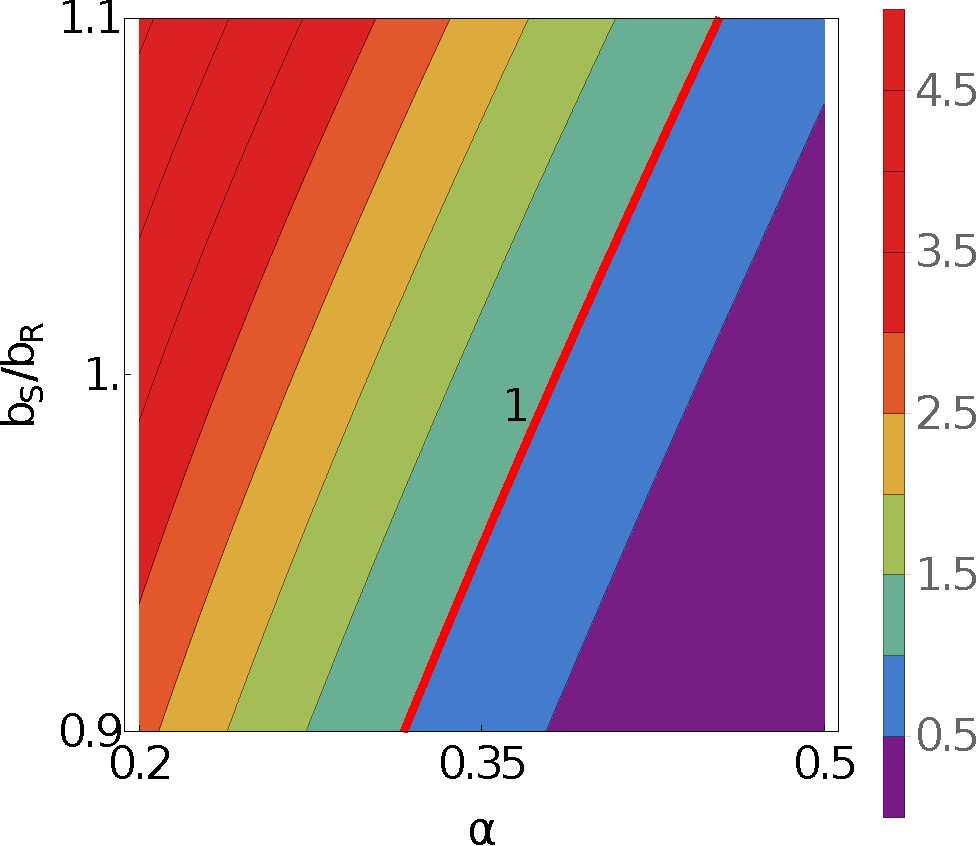
\includegraphics[width=\figwid]{../dev/graphics/poster/linear_contour.pdf}

      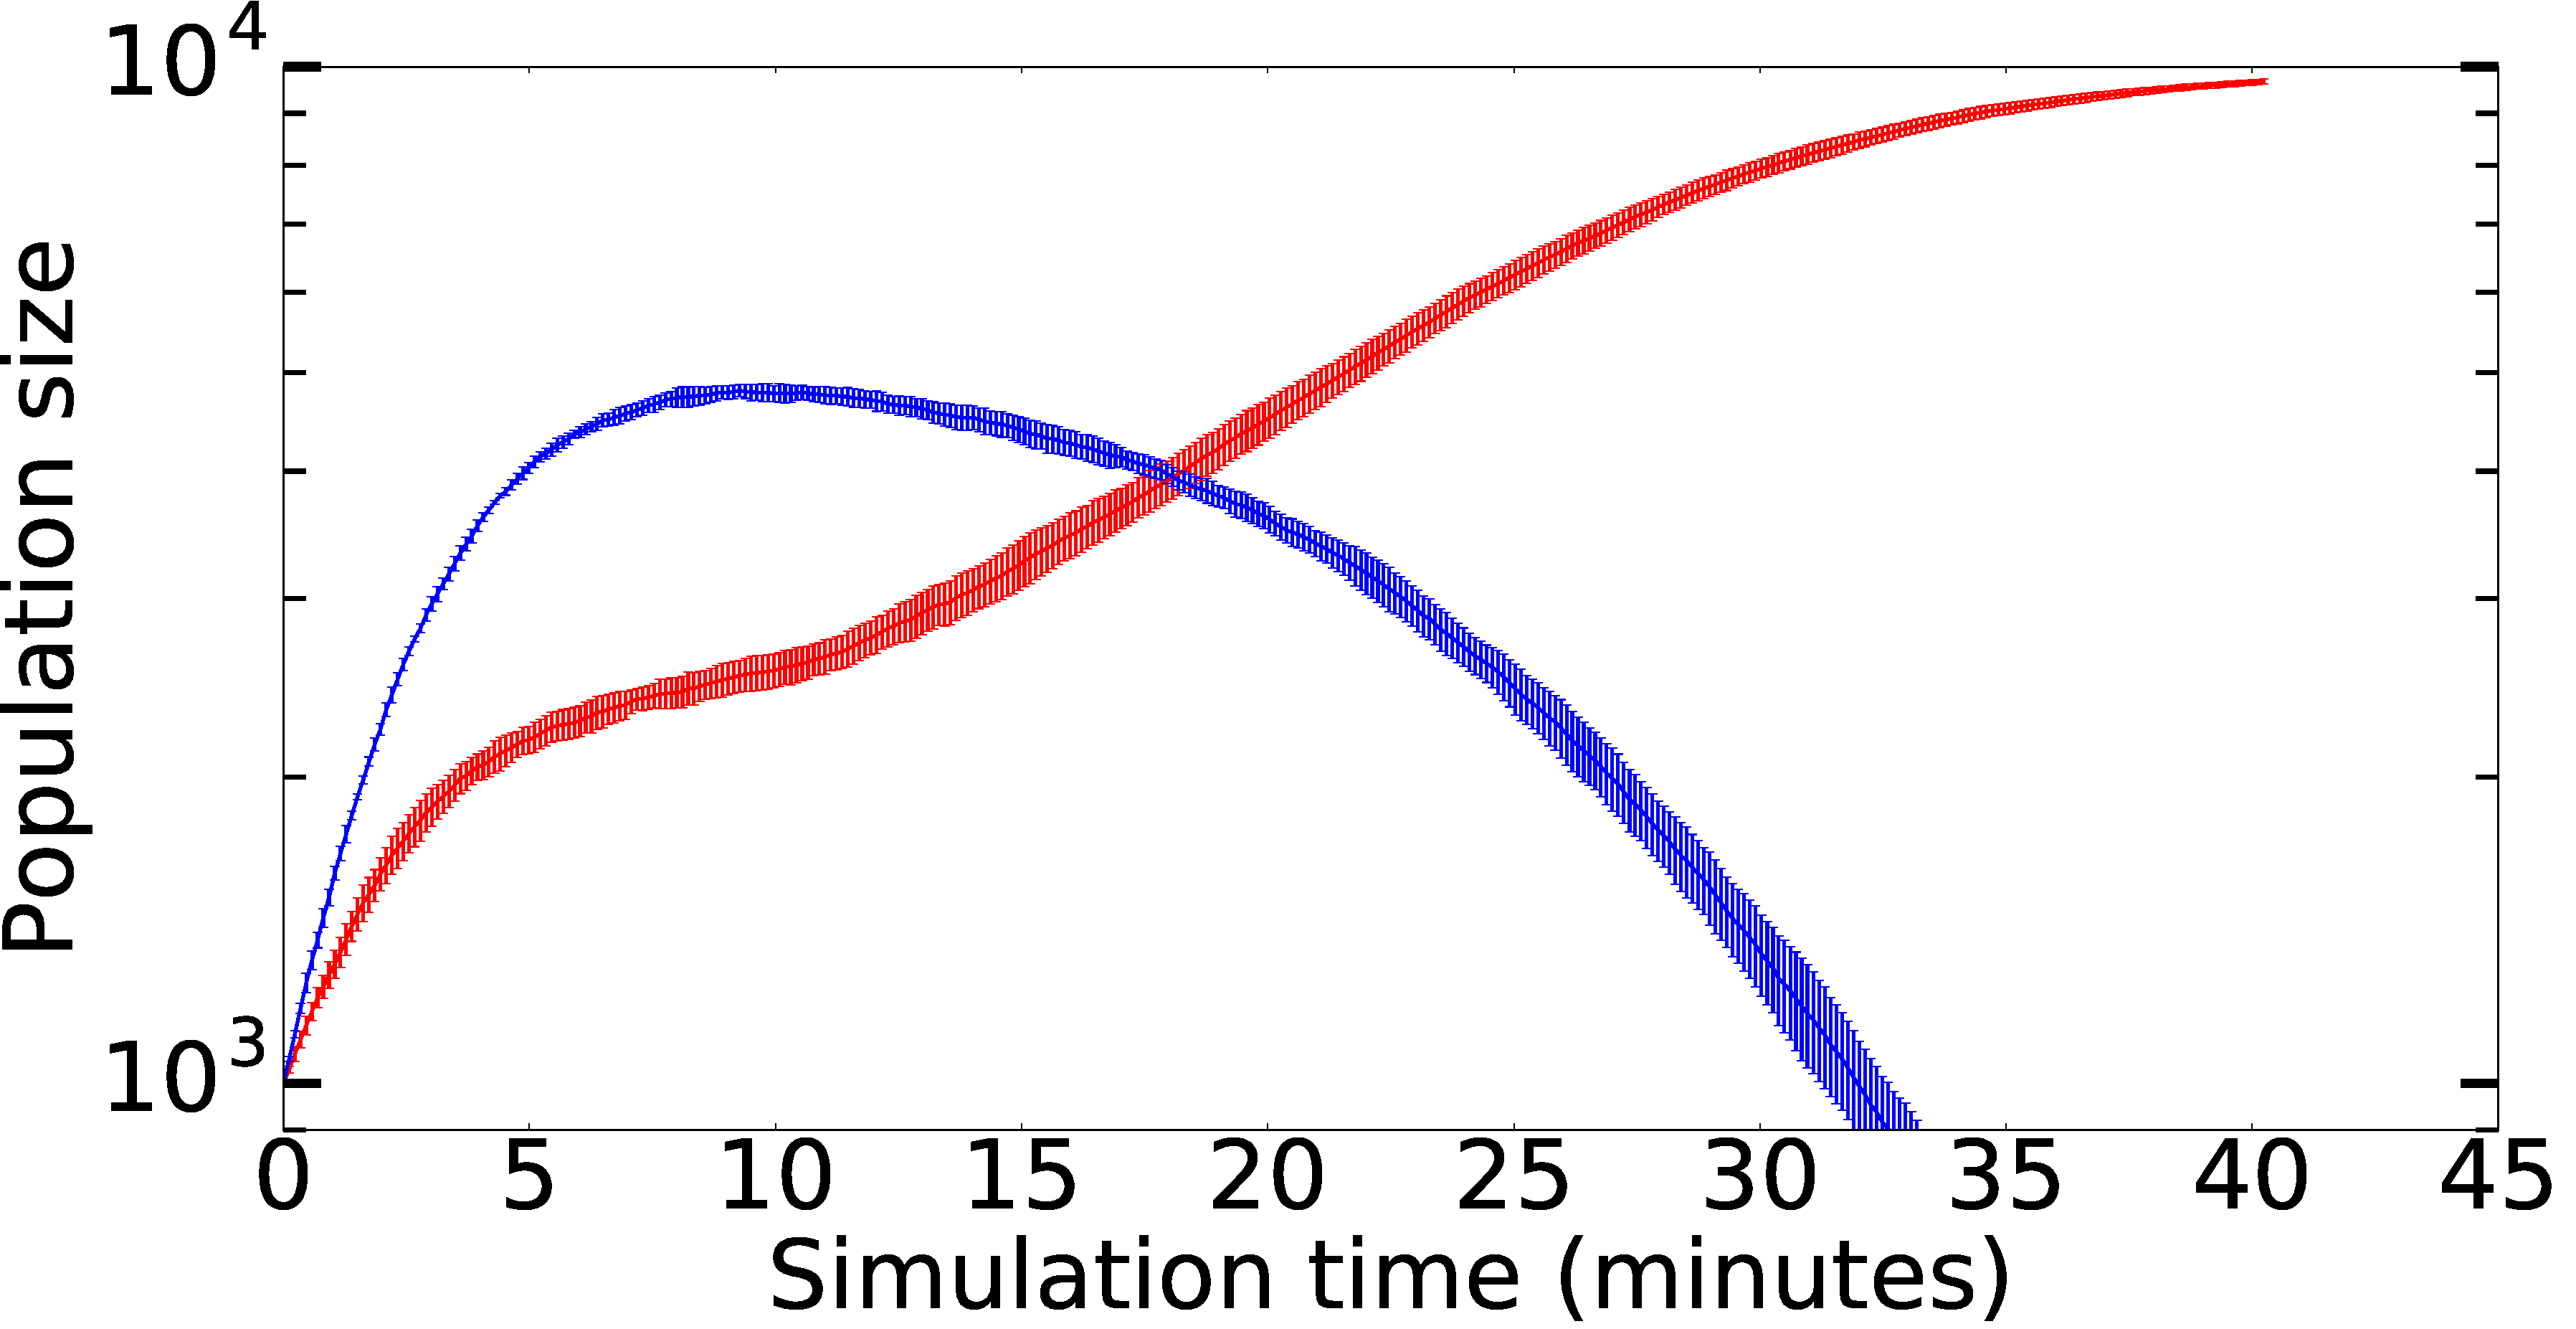
\includegraphics[width=\figwid]{../dev/graphics/poster/linear_pop.pdf}
    \end{center}

    \begin{columns}[t]
      \begin{column}{.2\onecolwid}
        \begin{center}
          Reactions
        \end{center}
        \begin{align*}
          S & \stackrel{b_S}{\rightarrow} 2S \\
          S \color{nred}+ P\color{black} & \stackrel{\alpha}{\rightarrow}  R \\[0.8ex]
          R &\stackrel{b_R}{\rightarrow} 2R \\
          R &\stackrel{\delta}{\rightarrow} \varnothing
        \end{align*}
      \end{column}
        \vrule
      \begin{column}{.6\onecolwid}
        \begin{center}
          Equations
        \end{center}

        \begin{align*}
          \frac{dS}{dt} & = \mu_1 \left(1 - \frac{S + R}{K}\right)S - \alpha
            \color{nred}\left( \frac{P}{P_0} \right)\color{black} S \\[0.8ex]
          \frac{dR}{dt} & = \mu_2 \left(1 - \frac{S + R}{K}\right)R + \
            \alpha \color{nred}\left( \frac{P}{P_0} \right)\color{black} S - \delta R \\[0.8ex]
          \color{nred} \frac{dP}{dt} & \color{nred} = -\alpha \left( \frac{P}{P_0} \right) S \color{black}
        \end{align*}
      \end{column}
    \end{columns}
  \end{block}
\end{column}


\vrule width 5pt
\begin{column}{1.5\sepwid}\end{column} % Empty spacer column
% ------------------------- Third column -------------------------
\begin{column}{\onecolwid}

  \setbeamercolor{block title}{fg=dblue,bg=white} % Colors of the block titles
  \begin{block}{Recycled $\alpha$}
  \setbeamercolor{block title}{fg=ngreen,bg=white} % Colors of the block titles
    \begin{center}
      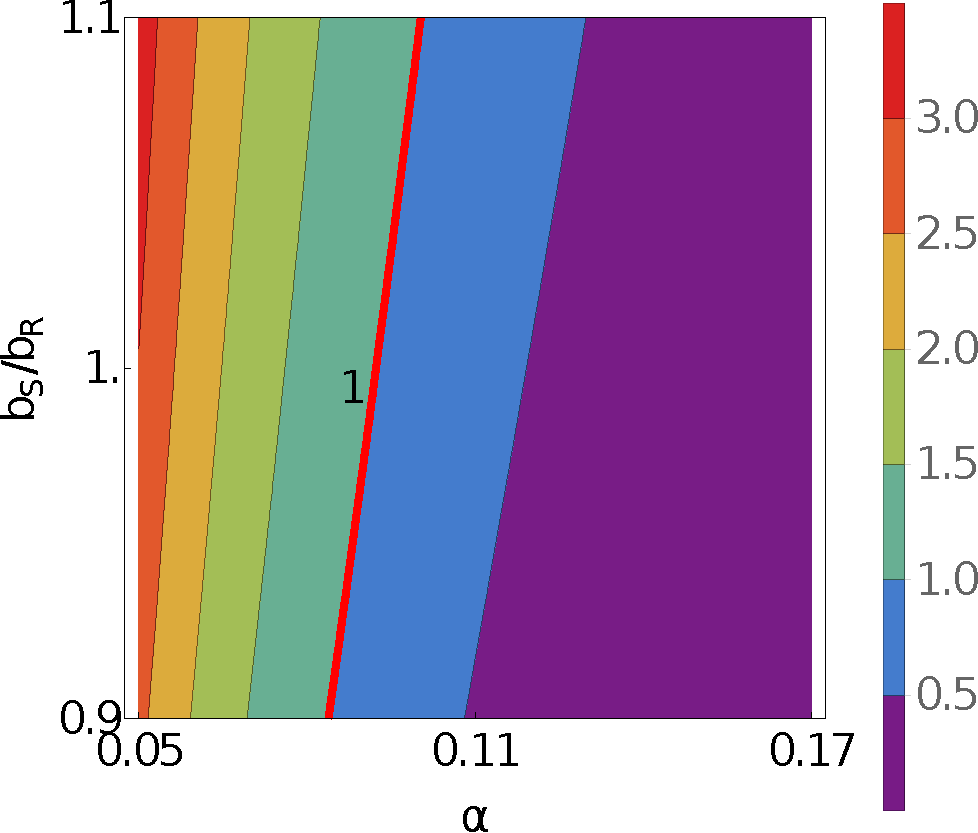
\includegraphics[width=\figwid]{../dev/graphics/poster/recycled_contour.pdf}

      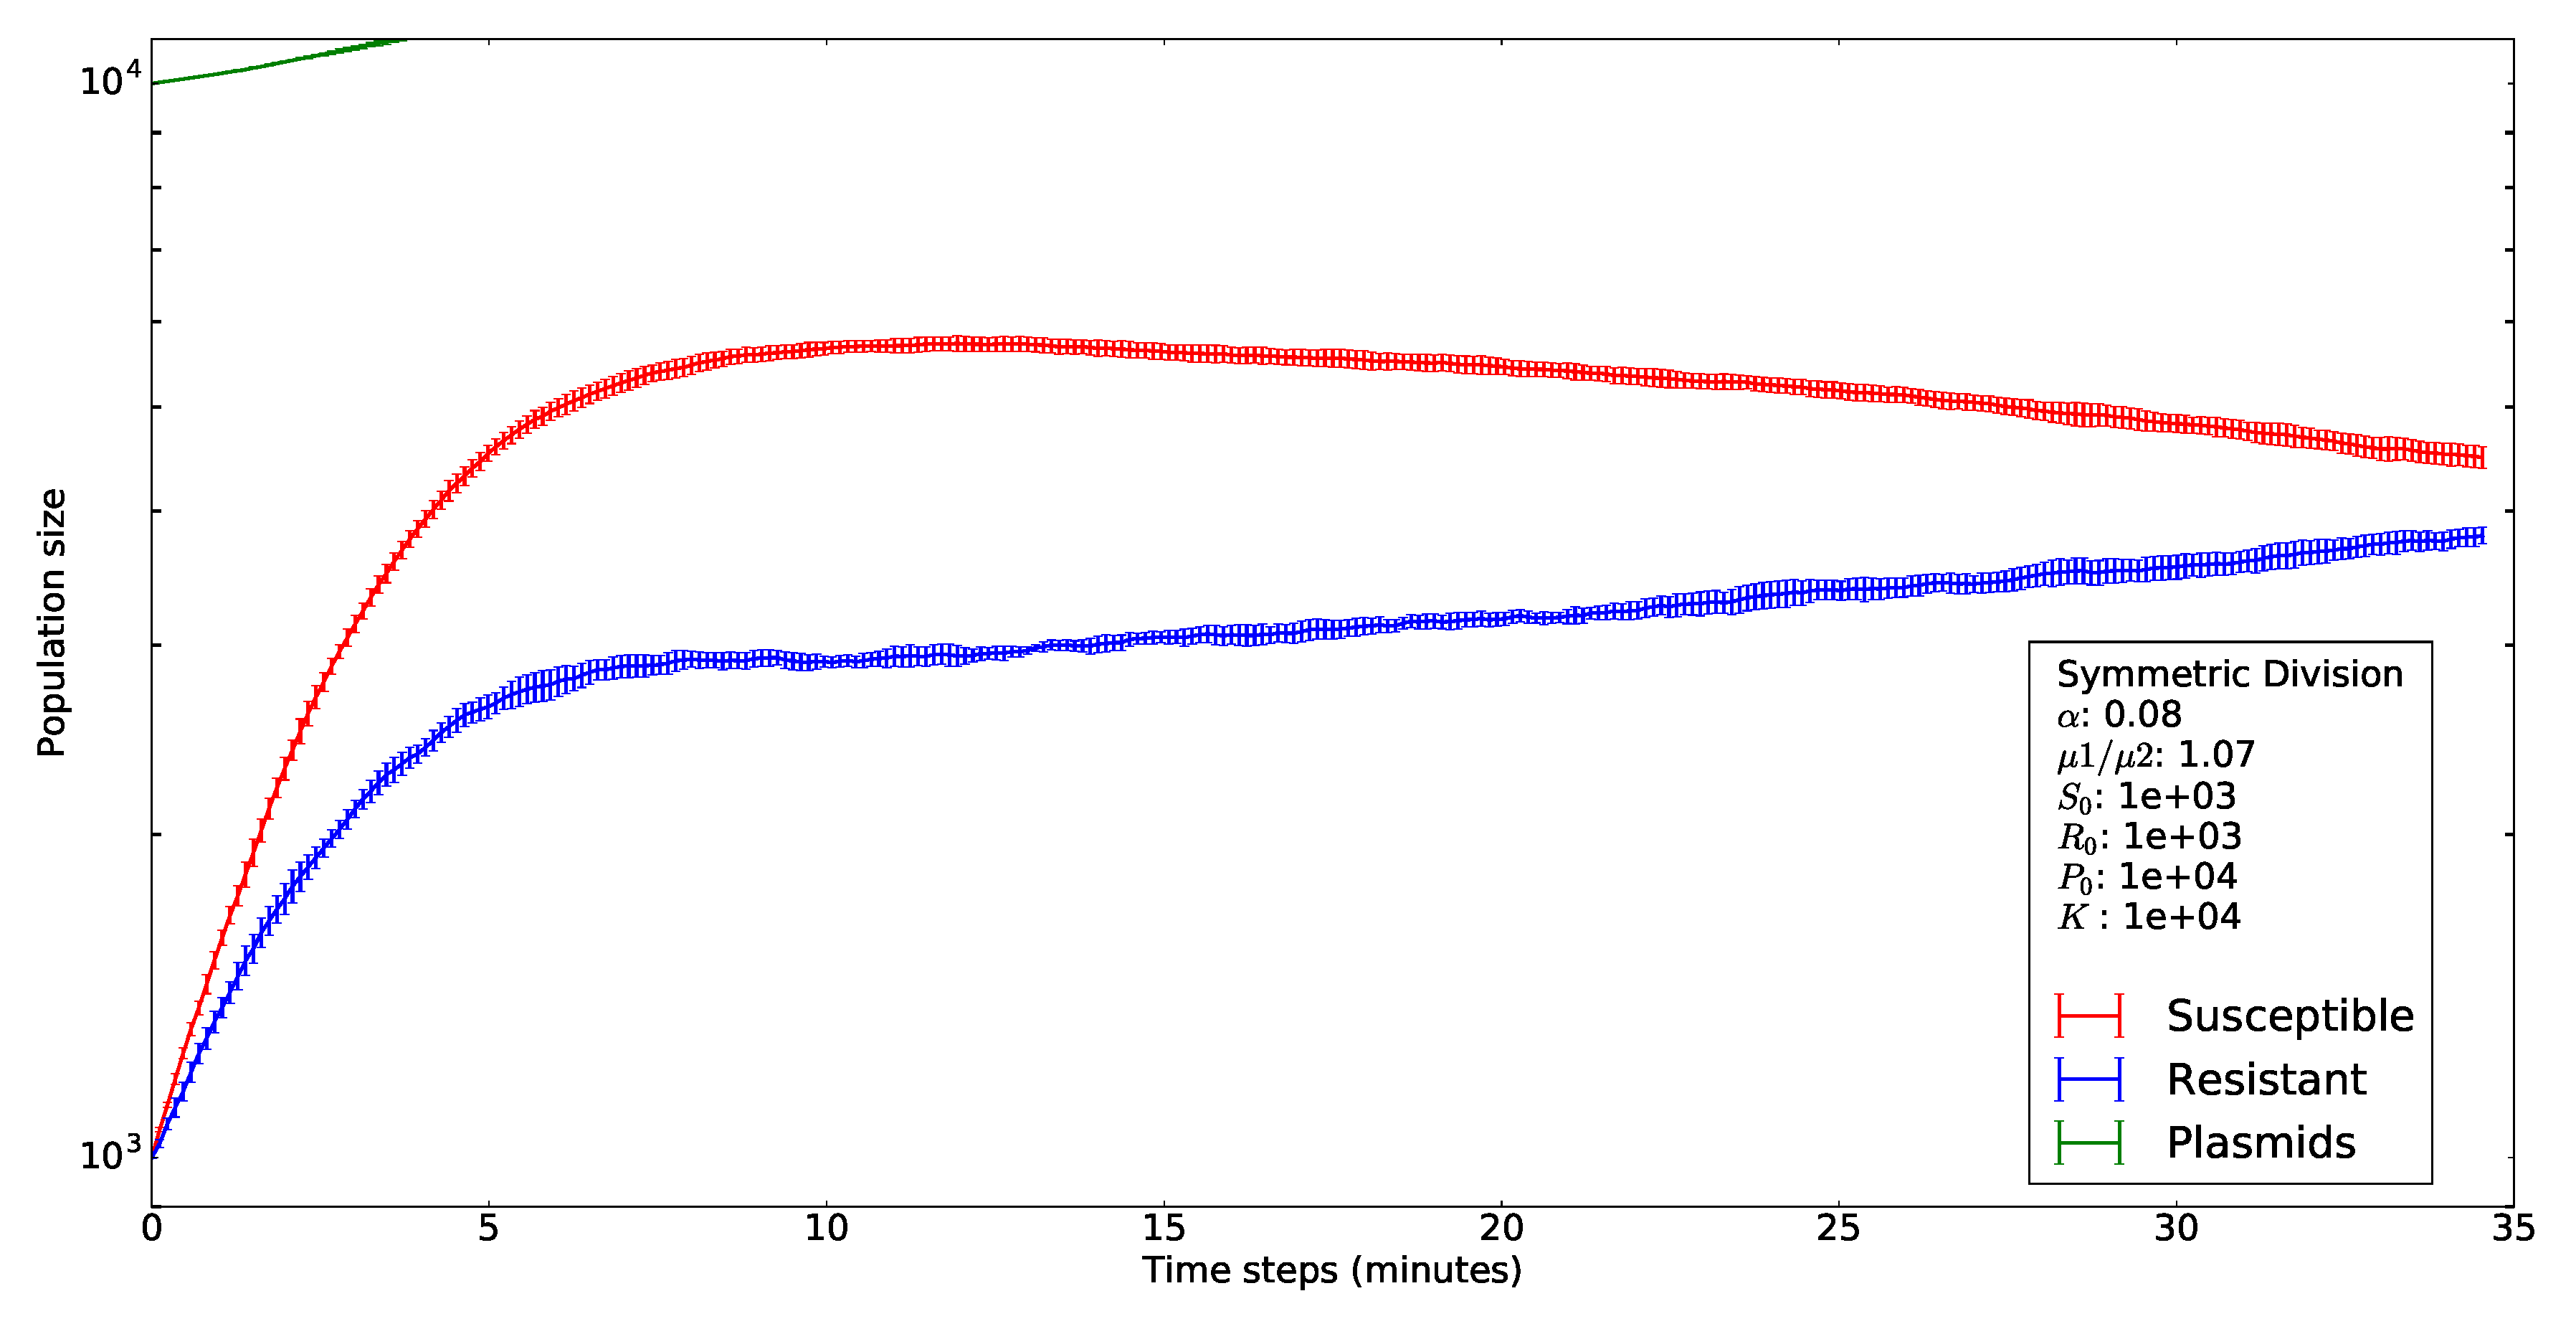
\includegraphics[width=\figwid]{../dev/graphics/poster/recycled_pop.pdf}
    \end{center}

    \begin{columns}[t]
      \begin{column}{.2\onecolwid}
        \begin{center}
          Reactions
        \end{center}
        \begin{align*}
          S &\stackrel{b_S}{\rightarrow} 2S \\
          S \color{nred}+ P\color{black} &\rightarrow  R \\
          R &\rightarrow 2R \\
          R &\rightarrow \varnothing \color{dblue} + P \color{black}
        \end{align*}
      \end{column}
        \vrule
      \begin{column}{.7\onecolwid}
        \begin{center}
          Equations
        \end{center}

        \begin{align*}
          \frac{dS}{dt} & = \mu_1 \left(1 - \frac{S + R}{K}\right)S - \alpha
          \color{nred} \left( \frac{P}{P_0} \right) \color{black} S +
            \color{dblue} + \mu_2 \left(1 - \frac{S + R}{K}\right)R \color{black}  \\[0.8ex]
        \frac{dR}{dt} & =  \alpha \color{nred} \left( \frac{P}{P_0} \right) \color{black} S  - \delta R \\[0.8ex]
        \color{nred} \frac{dP}{dt} & \color{nred} = -\alpha \left( \frac{P}{P_0} \right) S \color{dblue} + \delta R(t) \color{black}
        \end{align*}
      \end{column}
    \end{columns}
  \end{block}
\end{column}
% ----------------------------------------------------------------

% \begin{column}{\sepwid}\end{column} % Empty spacer column

\end{columns} % End of all the columns in the poster
\end{block}
\begin{block}

\begin{columns}[t] % The whole poster consists of three major columns, the second of which is split into two columns twice - the [t] option aligns each column's content to the top
% \begin{column}{\sepwid}\end{column} % Empty spacer column

% ------------------------- First column -------------------------
\begin{column}{\onecolwid}
  %-------------
  %	Conclusions
  %-------------
  \begin{alertblock}{Conclusions}
    \begin{itemize}
      \item Point
      \item Point
      \item Point
    \end{itemize}
    \vspace{.005\baselineskip}
  \end{alertblock}
\end{column}

% ----------------------------------------------------------------
\begin{column}{\sepwid}\end{column} % Empty spacer column

% ------------------------- Second column -------------------------
\begin{column}{\onecolwid}
  %-------------
  %	INTRODUCTION
  %-------------
  \begin{alertblock}{Future Work}
    \begin{itemize}
      \item Simulation on a lattice
      \item Adding antibiotics
      \item Asymmetric division
    \end{itemize}

    \vspace{.05ex}
  \end{alertblock}
\end{column}

\begin{column}{\sepwid}\end{column} % Empty spacer column

% ------------------------- Third column -------------------------
\begin{column}{.7\onecolwid}
  \begin{alertblock}{Acknowledgements/References}

      Thank you etc etc
  % \end{alertblock}
  %
  % \begin{alertblock}{References}

    \begin{itemize}
      \item Source 1
      \item Source 2
    \end{itemize}
  \end{alertblock}
\end{column}
% ----------------------------------------------------------------
% \begin{column}{\sepwid}\end{column} % Empty spacer column
\end{columns} % End of all the columns in the poster
\end{block}


\end{frame} % End of the enclosing frame

\end{document}
